\documentclass[tikz,border=2pt]{standalone}
\usepackage{amsmath,amssymb}
\usepackage{tikz}

\begin{document}
% A tree: connected and without cycles; with n vertices it has exactly n - 1 edges, and
% adding any edge creates a cycle while removing any edge disconnects it.
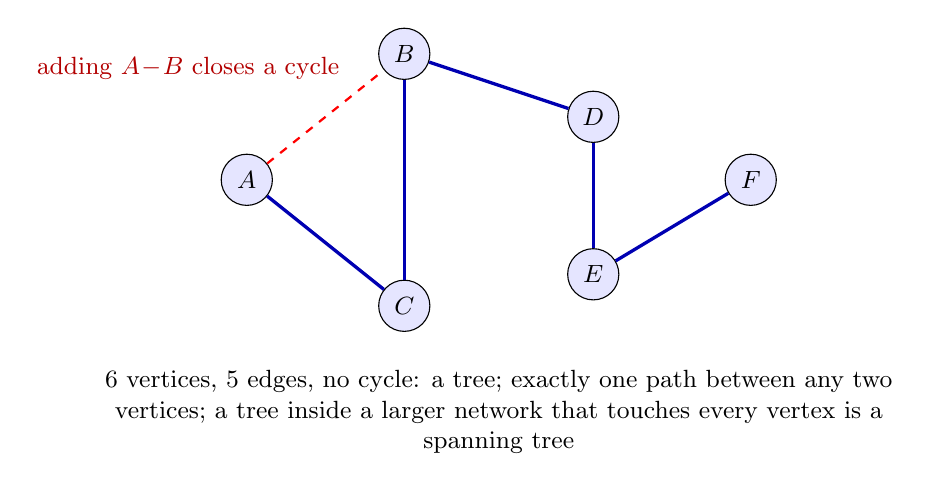
\begin{tikzpicture}[every node/.style={font=\small}, v/.style={draw, circle, fill=blue!10, minimum size=6.5mm, inner sep=0pt}]
	\node[v] (A) at (0,0) {$A$};
	\node[v] (B) at (2,1.6) {$B$};
	\node[v] (C) at (2,-1.6) {$C$};
	\node[v] (D) at (4.4,0.8) {$D$};
	\node[v] (E) at (4.4,-1.2) {$E$};
	\node[v] (F) at (6.4,0) {$F$};
	\foreach \a/\b in {A/C, C/B, B/D, D/E, E/F} {\draw[blue!70!black, very thick] (\a) -- (\b);}
	\draw[red, dashed, thick] (A) -- (B);
	\node[red!70!black, font=\small, anchor=south east] at (1.3,1.15) {adding $A\!-\!B$ closes a cycle};
	\node[anchor=north, align=flush center, text width=10cm] at (3.2,-2.3) {$6$ vertices, $5$ edges, no cycle: a tree; exactly one path between any two vertices; a tree inside a larger network that touches every vertex is a spanning tree};
\end{tikzpicture}
\end{document}
